% Include this to have simple page header/footer setup
%
% Use \pagestyle{NAME} to change to style named NAME
% empty - for title pages
% plain - for simple documents
% ...

\usepackage{tikz}   % used for producing vector graphics from a geometric/algebraic description
\usetikzlibrary{snakes}
\usetikzlibrary{matrix}
\usetikzlibrary{trees}
\usetikzlibrary{positioning,arrows}
\usetikzlibrary{decorations.pathmorphing}
\usetikzlibrary{decorations.markings}


\fancypagestyle{plain}{% 
\fancyhf{} % clear all header and footer fields
\fancyfoot[C]{\bfseries \thepage} % except the center
\renewcommand{\headrulewidth}{0pt}
\renewcommand{\footrulewidth}{0pt}}

\fancypagestyle{simple}{%
\fancyhf{} % clear all header and footer fields
\fancyhead[RO,LE]{\textsf{\footnotesize \thechapter--\thepage}}
\fancyhead[LO,RE]{\textsf{\footnotesize \leftmark}}
\fancyfoot[CO,CE]{\textsf{\footnotesize The Long-Baseline Neutrino Experiment}}}



% renewcommand this throughout the document to change the color; 
% done in lbne-sci-opp-main
\newcommand{\toccolor}{black}
\newcommand{\headrulecolor}{black}
\newcommand{\ChapterTabColor}{gray}

\fancypagestyle{mary}{%  THIS STANZA COULD USE SOME EXPLANATION 
\fancyhf{} % clear all header and footer fields
\fancyhead[RO,LE]{\textsf{\footnotesize \thechapter--\thepage}}
\fancyhead[LO,RE]{\textsf{\footnotesize \leftmark}}
\fancyfoot[CO,CE]{\textsf{\footnotesize The Long-Baseline Neutrino Experiment}}
%\fancyfoot[CO,CE]{\includegraphics[scale=0.25]{lbnelogo.png}}
\fancyfoot[LE]{%
\setlength{\unitlength}{1mm}
  \begin{tikzpicture}[remember picture,overlay] %  THIS COULD USE SOME EXPLANATION 
    \draw[fill=\ChapterTabColor,\ChapterTabColor] (18,20) rectangle (22,21);
    \draw[fill=\ChapterTabColor,\ChapterTabColor] (18,18.5) rectangle (22,19.5);
    \draw[fill=\ChapterTabColor,\ChapterTabColor] (18,17) rectangle (22,18);
    \node at (17,0) {\includegraphics[scale=0.3]{lbnelogo.png}};
   \end{tikzpicture}
}
\fancyfoot[RO]{%
\setlength{\unitlength}{1mm}
  \begin{tikzpicture}[remember picture,overlay]
    \draw[fill=\ChapterTabColor,\ChapterTabColor] (-18,20) rectangle (-22,21);
    \draw[fill=\ChapterTabColor,\ChapterTabColor] (-18,18.5) rectangle (-22,19.5);
    \draw[fill=\ChapterTabColor,\ChapterTabColor] (-18,17) rectangle (-22,18);
    \node at (-17,0) {\includegraphics[scale=0.3]{lbnelogo.png}};
   \end{tikzpicture}
}
\renewcommand{\headrulewidth}{4pt}
\renewcommand{\headrule}{{\color{\headrulecolor}%
\hrule width\headwidth height\headrulewidth \vskip-\headrulewidth}}

}


\fancypagestyle{glossy}{%
\fancyhf{} % clear all header and footer fields

\fancyhead[RO,LE]{\textsf{\footnotesize \bfseries \thepage}}
\fancyhead[CE]{\textcolor{\headrulecolor}{\textsf{\footnotesize \bfseries \thechapter~\leftmark}}}
\fancyhead[CO]{\textcolor{\headrulecolor}{\textsf{\footnotesize \bfseries \thechapter\ifnum\value{section}>0 .\arabic{section} \fi~\rightmark}}}
\fancyfoot[CO,CE]{\textsf{\footnotesize \bfseries The Long-Baseline Neutrino Experiment}}
% Not sure why the xoff numbers are asymmetric to get the same size
% tabs showing, but they are.  -0.7 and 0.8.  Change them only if you
% know what you are doing.
\fancyfoot[LE]{\margintabs{3}{1.5}{-0.7}{18}{-4}{1}{1.5}}
\fancyfoot[RO]{\margintabs{3}{1.5}{0.8}{18}{4}{1}{1.5}}
\renewcommand{\headrulewidth}{1pt}
\renewcommand{\headrule}{{\color{\headrulecolor}%
\hrule width\headwidth height\headrulewidth \vskip-\headrulewidth}}

}

\fancypagestyle{references}{%
\fancyhf{} % clear all header and footer fields
\fancyhead[RO,LE]{\textsf{\footnotesize \bfseries \thepage}}
\fancyhead[LO,RE]{\textsf{\footnotesize References}}
\fancyfoot[CO,CE]{\textsf{\footnotesize \bfseries The Long-Baseline Neutrino Experiment}}
%\fancyfoot[CO,CE]{\includegraphics[scale=0.25]{lbnelogo.png}}
\fancyfoot[LE]{\margintabs{3}{1.5}{-0.8}{18}{-4}{1}{1.5}}
\fancyfoot[RO]{\margintabs{3}{1.5}{0.8}{18}{4}{1}{1.5}}
\renewcommand{\headrulewidth}{1pt}
\renewcommand{\headrule}{{\color{\headrulecolor}%
\hrule width\headwidth height\headrulewidth \vskip-\headrulewidth}}

}
\fancypagestyle{acknowledgement}{%
\fancyhf{} % clear all header and footer fields
\fancyhead[RO,LE]{\textsf{\footnotesize \bfseries \thepage}}
\fancyhead[LO,RE]{\textsf{\footnotesize Acknowledgements}}
\fancyfoot[CO,CE]{\textsf{\footnotesize \bfseries The Long-Baseline Neutrino Experiment}}
%\fancyfoot[CO,CE]{\includegraphics[scale=0.25]{lbnelogo.png}}
\fancyfoot[LE]{\margintabs{3}{1.5}{-0.8}{18}{-4}{1}{1.5}}
\fancyfoot[RO]{\margintabs{3}{1.5}{0.8}{18}{4}{1}{1.5}}
\renewcommand{\headrulewidth}{1pt}
\renewcommand{\headrule}{{\color{\headrulecolor}%
\hrule width\headwidth height\headrulewidth \vskip-\headrulewidth}}

}

\fancypagestyle{wiggles}{%
\fancyhf{} % clear all header and footer fields
\fancyhead[EC,OC]{
\leftmark\\
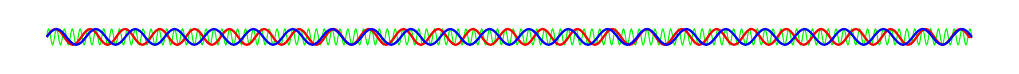
\begin{tikzpicture}
  \node (a) at (0,0) {};
  \node (b) at (12,0) {};
  \draw[thin,green,snake=coil,segment aspect=0,segment amplitude=1mm,segment length=1mm] (a) -- (b);
  \draw[thick,red,snake=coil,segment aspect=0,segment amplitude=1mm,segment length=4.42mm]  (a) -- (b);
  \draw[thick,blue,snake=coil,segment aspect=0,segment amplitude=1mm,segment length=5mm] (a) -- (b);
\end{tikzpicture}}
\fancyfoot[C]{\bfseries \thepage}
\renewcommand{\headrulewidth}{0pt}
\renewcommand{\footrulewidth}{0pt}}

